\documentclass[border=15pt, multi, tikz]{standalone}
\usepackage{import}
\usepackage{etoolbox}
\usepackage{graphicx}
\usepackage{svg}
\usepackage{colortbl}

\usetikzlibrary{positioning,matrix,fit}
\usetikzlibrary{3d} %for including external image
\usetikzlibrary{decorations,shapes}
\usetikzlibrary{decorations.shapes}
\usetikzlibrary{decorations.markings}
\usetikzlibrary{decorations.pathreplacing}
\usetikzlibrary{backgrounds}
\usetikzlibrary{calc}
\usetikzlibrary{arrows.meta,arrows}
\graphicspath{{image/}}

\colorlet{inputCell}{red!30}
\colorlet{cellColor}{green!80!black}

\tikzset{%
  % Specifications for style of nodes:
    >={Latex[width=2mm,length=3mm]},
    baseChannel/.style = {rectangle,draw,fill=white!80},
    inputChannel/.style = {baseChannel,minimum width=8.8em, minimum height=8.8em},
    kernelChannel/.style = {baseChannel,minimum width=3.75em, minimum height=3.75em},
    convResChannel/.style = {baseChannel,minimum width=6.2em, minimum height=6.2em},
    matrixCell/.style={draw, minimum width=1.2em, minimum height=1.25em, outer sep=0, inner sep=0, anchor=center},
    matrixFull/.style={matrix of nodes, nodes in empty cells, nodes=matrixCell, row sep=-\pgflinewidth},
}

\begin{document}
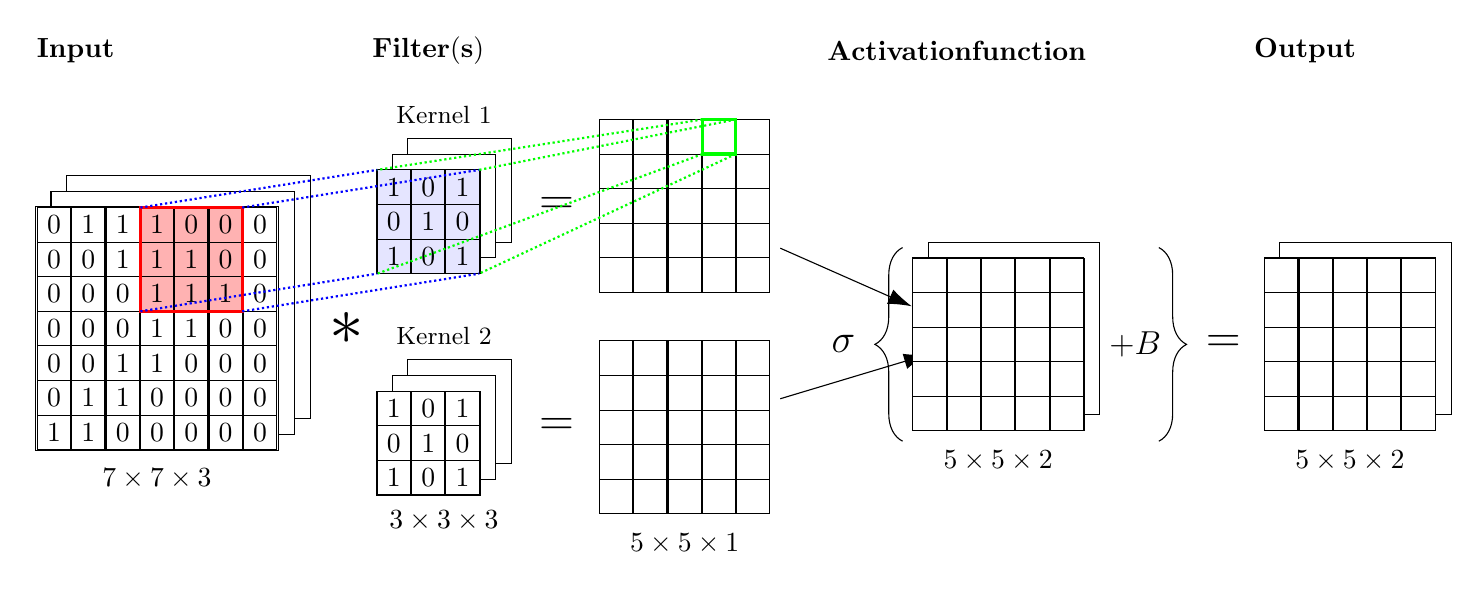
\begin{tikzpicture}
	\node [inputChannel] (input-1) {};
	\node [inputChannel, shift={(-0.2,-0.2)}] (input-2) at (input-1) {};
	\node [inputChannel, shift={(-0.2,-0.2)}] (input-3) at (input-2) {};
	\matrix (input) at (input-3) [matrixFull]
	{
		0 & 1 & 1 & |[fill=inputCell]| 1 & |[fill=inputCell]| 0 & |[fill=inputCell]| 0 & 0\\
		0 & 0 & 1 & |[fill=inputCell]| 1 & |[fill=inputCell]| 1 & |[fill=inputCell]| 0 & 0\\
		0 & 0 & 0 & |[fill=inputCell]| 1 & |[fill=inputCell]| 1 & |[fill=inputCell]| 1 & 0\\
		0 & 0 & 0 & 1 & 1 & 0 & 0\\
		0 & 0 & 1 & 1 & 0 & 0 & 0\\
		0 & 1 & 1 & 0 & 0 & 0 & 0\\
		1 & 1 & 0 & 0 & 0 & 0 & 0\\
	};
	\draw[very thick, red] (input-1-4.north west) rectangle (input-3-6.south east);
	
	\node [anchor=south west,yshift=4.5em] at (input.north west) (inputLabel) {$\bf Input$};
	\node [below= of input-5-4.south] (lm) {$7\times7\times3$};
	\node[right = 1.2em of input] (str) {\Huge $*$};
	
	
	\node [kernelChannel, right=1.2em of str, yshift=5em] (kernel-1-1) {};
	\node [kernelChannel, shift={(-0.2,-0.2)}] (kernel-1-2) at (kernel-1-1) {};
	\node [kernelChannel, shift={(-0.2,-0.2)}] (kernel-1-3) at (kernel-1-2) {};
	\matrix (kernel1) at (kernel-1-3) [matrixFull,nodes={fill=blue!10}]
	{
		1 & 0 & 1 \\
		0 & 1 & 0 \\
		1 & 0 & 1 \\
	};
	\node [above = .75em of kernel-1-2] {\small Kernel 1};
	
	\node [right = 1.2em of kernel-1-2] (eq) {\bf\LARGE$=$};
	\matrix (conv1) [right=0.2em of eq, matrixFull]
	{
		& & & & \\
		& & & & \\
		& & & & \\
		& & & & \\
		& & & & \\
	};
	
	
	\node [kernelChannel, right=1.2em of str, yshift=-3em] (kernel-2-1) {};
	\node [kernelChannel, shift={(-0.2,-0.2)}] (kernel-2-2) at (kernel-2-1) {};
	\node [kernelChannel, shift={(-0.2,-0.2)}] (kernel-2-3) at (kernel-2-2) {};
	\matrix (kernel2) at (kernel-2-3) [matrixFull]
	{
		1 & 0 & 1 \\
		0 & 1 & 0 \\
		1 & 0 & 1 \\
	};
	\node [above = .75em of kernel-2-2] {\small Kernel 2};
	\node [below=.75em of kernel-2-2] {$3\times3\times3$};
	
	\node [right = 1.2em of kernel-2-2] (eq) {\bf\LARGE$=$};
	\matrix (conv2) [right=0.2em of eq, matrixFull]
	{
		& & & & \\
		& & & & \\
		& & & & \\
		& & & & \\
		& & & & \\
	};
	\node [] at (inputLabel -| kernel1) {$\bf Filter(s)$};
	\node [below=0em of conv2] {$5\times5\times1$};

	\node [convResChannel, right=20em of str] (convRes1) {};
	\draw[->] (conv2) -- (convRes1);
	\node [convResChannel, shift={(-0.2,-0.2)}] (convRes2) at (convRes1) {};
	\draw[->] (conv1) -- (convRes2);
	\matrix (convRes) at (convRes2) [matrixFull]
	{
		& & & & \\
		& & & & \\
		& & & & \\
		& & & & \\
		& & & & \\
	};
	\node [below=0em of convRes] {$5\times5\times2$};
	
	\node[right=2em of convRes] (reluEnd) {};
	\draw [decorate,decoration={mirror,brace,amplitude=10pt}] (convRes.north west) -- (convRes.south west) node [black,midway,xshift=-.75cm] {\Large $\sigma$};
	\draw [decorate,decoration={brace,amplitude=10pt}] (convRes.north -| reluEnd) -- (convRes.south -| reluEnd) node [black,midway,xshift=-.3cm] {\large $+B$};
	
	\node [xshift=-1.5em] at (inputLabel -| convRes) {$\bf Activation function$};
	\node [right = 1em of reluEnd] (eq) {\LARGE$=$};
	
	\node [convResChannel, right=4em of reluEnd, yshift=0.2cm] (ouput1) {};
	\node [convResChannel, shift={(-0.2,-0.2)}] (ouput2) at (ouput1) {};
	\matrix (ouput) at (ouput2) [matrixFull]
	{
		& & & & \\
		& & & & \\
		& & & & \\
		& & & & \\
		& & & & \\
	};
	\node [anchor=east] at (inputLabel -| ouput1) {$\bf Output$};
	\node [below=0em of ouput] {$5\times5\times2$};

	\draw[very thick, green] (conv1-1-4.north west) rectangle (conv1-1-4.south east);

	\draw[densely dotted, blue, thick] (input-1-4.north west) -- (kernel1-1-1.north west);
	\draw[densely dotted, blue, thick] (input-3-4.south west) -- (kernel1-3-1.south west);
	\draw[densely dotted, blue, thick] (input-1-6.north east) -- (kernel1-1-3.north east);
	\draw[densely dotted, blue, thick] (input-3-6.south east) -- (kernel1-3-3.south east);

	\draw[densely dotted, green, thick] (conv1-1-4.north west) -- (kernel1-1-1.north west);
	\draw[densely dotted, green, thick] (conv1-1-4.south west) -- (kernel1-3-1.south west);
	\draw[densely dotted, green, thick] (conv1-1-4.north east) -- (kernel1-1-3.north east);
	\draw[densely dotted, green, thick] (conv1-1-4.south east) -- (kernel1-3-3.south east);

\end{tikzpicture}
\end{document}